\documentclass[12pt,a4paper]{article}
\usepackage[utf8]{inputenc}
\usepackage[spanish,es-tabla]{babel}
\usepackage{geometry}
\usepackage{graphicx}
\usepackage{multirow}
\usepackage{tabularx}
\usepackage{mathptmx}
\usepackage{fancyhdr}
\usepackage{array}
\usepackage[table]{xcolor}
\usepackage{titlesec}
\usepackage{setspace}
\usepackage{microtype}
\usepackage{lastpage}
\usepackage{booktabs}
\usepackage{enumitem}
\usepackage{amsmath}
\usepackage{amsfonts}
\usepackage{amssymb}

\graphicspath{{images/}{../images/}{../../images/}{./}}

\geometry{
    top=4.7cm,
    bottom=2.5cm,
    left=2.5cm,
    right=2.5cm,
    headheight=3.9cm,
    headsep=0.4cm
}

\setstretch{1.15}
\setlength{\parindent}{0pt}
\setlength{\parskip}{0.45em}
\setlength{\tabcolsep}{4pt}

\titleformat{\section}
  {\normalfont\fontsize{12}{14.5}\bfseries}{\thesection.}{0.6em}{\uppercase}
\titlespacing*{\section}
  {0pt}{1.8ex plus 0.4ex minus 0.2ex}{0.6ex plus 0.2ex}

\titleformat{\subsection}
  {\normalfont\fontsize{11.5}{13.5}\bfseries}{\thesubsection.}{0.5em}{}
\titlespacing*{\subsection}
  {0pt}{1.4ex plus 0.3ex minus 0.1ex}{0.4ex plus 0.1ex}

\titleformat{\subsubsection}
  {\normalfont\fontsize{10.5}{12.5}\bfseries\itshape}{\thesubsubsection.}{0.4em}{}
\titlespacing*{\subsubsection}
  {0pt}{1.1ex plus 0.2ex minus 0.1ex}{0.3ex plus 0.1ex}

\newcolumntype{Y}{>{\centering\arraybackslash}X}
\newcolumntype{L}{>{\raggedright\arraybackslash}X}
\newcolumntype{C}{>{\centering\arraybackslash}X}

\definecolor{headerred}{RGB}{180, 0, 0}
\definecolor{darkred}{RGB}{140, 0, 0}
\definecolor{lightgraybg}{RGB}{248, 248, 248}
\definecolor{tableheader}{RGB}{232, 238, 246}

\newcommand{\docCodigo}{TI-SIGE-ENT-S3-004}
\newcommand{\docVersion}{1.0}
\newcommand{\docProceso}{DESARROLLO FRONTEND / CLIENTE WEB SPA}
\newcommand{\docElaboracion}{14/09/2026}
\newcommand{\docRevision}{APROBADO POR LÍDER TÉCNICO}
\newcommand{\docTitulo}{CLIENTE BASE EN REACT 19 + TYPESCRIPT + VITE + TAILWIND CSS}
\newcommand{\docOrganizacion}{FACULTAD DE INGENIERÍA EN SISTEMAS, ELECTRÓNICA E INDUSTRIAL}
\newcommand{\docSubOrganizacion}{CARRERA DE INGENIERÍA DE SOFTWARE}

\newcommand{\encabezadofrecuente}{%
    \renewcommand{\arraystretch}{1.15}%
    \noindent\makebox[\textwidth][c]{%
    \begin{tabularx}{\textwidth}{|>{\centering\arraybackslash}m{2.8cm}|Y|>{\centering\arraybackslash}m{4.8cm}|}
        \hline
        \multirow{4}{2.8cm}{\centering\raisebox{-1.15cm}{
\includegraphics[width=2.5cm,height=2.0cm,keepaspectratio]{logo.png}}}
        & \textbf{\fontsize{9}{11}\selectfont \docOrganizacion} 
        & \textbf{\fontsize{8}{10}\selectfont CÓDIGO:} \fontsize{8}{10}\selectfont \docCodigo \\
        \cline{3-3}
        & \textbf{\fontsize{8.5}{10.5}\selectfont \docSubOrganizacion} 
        & \textbf{\fontsize{8}{10}\selectfont VERSIÓN:} \fontsize{8}{10}\selectfont \docVersion \\
        \cline{2-3}
        & \textbf{\fontsize{8}{10}\selectfont PROCESO:} \fontsize{8}{10}\selectfont \docProceso 
        & \textbf{\fontsize{8}{10}\selectfont ELABORACIÓN:} \fontsize{8}{10}\selectfont \docElaboracion \\
        \cline{2-3}
        & \textbf{\fontsize{8.5}{10.5}\selectfont \docTitulo} 
        & \textbf{\fontsize{8}{10}\selectfont ÚLTIMA REVISIÓN:} \fontsize{8}{10}\selectfont \textbf{\textcolor{darkred}{\docRevision}} \\
        \hline
    \end{tabularx}%
    }%
}

\pagestyle{fancy}
\fancyhf{}
\fancyhead[C]{\encabezadofrecuente}
\fancyfoot[C]{\fontsize{10}{12}\selectfont Página \thepage\ de \pageref{LastPage}}
\renewcommand{\headrulewidth}{0pt}

\begin{document}

\section{Título}
\textbf{Denominación del Entregable:} Configuración del Cliente Web Base: React 19, TypeScript, Vite, Tailwind CSS y Sistema de Navegación

\vspace{0.15cm}
\noindent
\textbf{Ficha Técnica de Identificación:}
\begin{itemize}[leftmargin=1.5em, itemsep=1.5pt, topsep=1.5pt]
    \item \textbf{Código Documental:} \docCodigo \quad | \quad \textbf{Versión:} \docVersion
    \item \textbf{Institución:} Universidad Técnica de Ambato (UTA) -- FISEI
    \item \textbf{Carrera:} Ingeniería de Software (Séptimo Semestre "A")
    \item \textbf{Módulo Académico:} Gestión de Proyectos de Software
    \item \textbf{Docente Tutor:} Ing. Paulo Torres
    \item \textbf{Fecha de Elaboración:} \docElaboracion \quad | \quad \textbf{Estado:} \textbf{\textcolor{darkred}{Completado / En Auditoría}}
    \item \textbf{Período de Ejecución:} Semana 3 (08/09/2026 al 14/09/2026 -- EDT 3.4: 5 días laborables, 40h)
\end{itemize}

\section{Introducción}
La interfaz de usuario del sistema \textbf{SIGE} debe proporcionar una experiencia moderna, fluida y adaptativa a los docentes y autoridades de la FISEI. Para lograr tiempos de carga instantáneos y alta confiabilidad en tipado estático, se adoptó el stack conformado por **React 19**, **TypeScript**, **Vite** y **Tailwind CSS**.

Este entregable describe la inicialización del proyecto cliente \texttt{SIGE.ClientApp}, la configuración del diseño atómico con la paleta de colores institucional de la UTA, la integración del enrutador SPA (*Single Page Application*) con rutas protegidas según roles, y la capa cliente para la comunicación HTTP con la WebAPI.

\section{Objetivo}

\subsection{Objetivo General}
Construir la arquitectura base del cliente frontend en React 19 con TypeScript y Vite, estableciendo el sistema de componentes visuales, el manejo de rutas protegidas y la integración con el API de autenticación.

\subsection{Objetivos Específicos}
\begin{itemize}[leftmargin=1.5em, itemsep=1.5pt, topsep=1.5pt]
    \item Inicializar el bundle con Vite garantizando compilación ultra-rápida (HMR) y tipado estricto en TypeScript.
    \item Diseñar la biblioteca de tokens CSS institucional (Rojo UTA \texttt{\#B40000}, Azul Oscuro \texttt{\#0C2340}, Fondo \texttt{\#F8FAFC}).
    \item Implementar el enrutador con \texttt{react-router-dom} y guardas de navegación (*Guards*) para roles docentes y directivos.
    \item Crear los componentes base reutilizables: Navbar, Sidebar colapsable, Modal institucional y alertas Toast.
\end{itemize}

\section{Alcance}

\subsection{Alcance Incluido}
Proyecto SPA \texttt{SIGE.ClientApp} operativo en el puerto 5173, pantalla de inicio de sesión con validación institucional, Dashboard general y cliente Axios con interceptores JWT.

\subsection{Límites y Exclusiones}
No incluye el editor TipTap (EDT 3.6) ni la matriz de actividades (EDT 3.9).

\section{Definiciones}
\begin{itemize}[leftmargin=1.5em, itemsep=2pt, topsep=2pt]
    \item \textbf{Vite:} Herramienta de compilación frontend basada en módulos ES nativos para desarrollo ultra-veloz.
    \item \textbf{Route Guard:} Componente de protección de rutas que verifica si el usuario autenticado posee el rol requerido.
\end{itemize}

\section{Responsabilidades}
\begin{itemize}[leftmargin=1.5em, itemsep=2pt, topsep=2pt]
    \item \textbf{Andrea Vasquez (Frontend / QA):} Estructura de carpetas, configuración de Vite, rutas y consumo de servicios con Axios.
    \item \textbf{Heidy Villavicencio (Analista / UI-UX):} Maquetación responsiva y alineación con los wireframes de Figma.
    \item \textbf{Ing. Paulo Torres (Docente Tutor):} Validación de usabilidad y aprobación del cliente base.
\end{itemize}

\section{Método, Políticas y Contenidos}
Desarrollo basado en componentes funcionales de React 19 con Hooks nativos y TypeScript estricto sin tipo \texttt{any}. Los estilos visuales se gestionan mediante clases utilitarias de Tailwind CSS evitando CSS arbitrario disperso.

\begin{figure}[htbp]
    \centering
    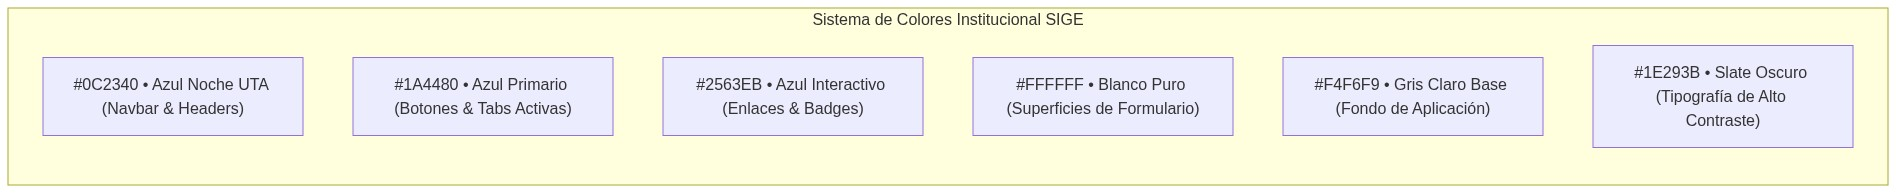
\includegraphics[width=0.85\textwidth,keepaspectratio]{images/s2_05_paleta_colores.png}
    \caption{Paleta de Colores Institucional FISEI UTA y Tokens de Diseño en Tailwind CSS.}
    \label{fig:paleta_colores}
\end{figure}

\section{Descripción de actividades}

\subsection{Estructura del Proyecto y Enrutador Modular}
Se organizó el directorio bajo diseño atómico en \texttt{src/components}, \texttt{src/pages} y \texttt{src/routes}, implementando \texttt{react-router-dom} con rutas protegidas por roles.

\subsection{Configuración de Interceptor Axios para JWT}
El interceptor inyecta automáticamente el token almacenado en \texttt{localStorage} en todas las peticiones salientes hacia la WebAPI:
\begin{verbatim}
api.interceptors.request.use((config) => {
  const token = localStorage.getItem('sige_token');
  if (token) {
    config.headers.Authorization = `Bearer ${token}`;
  }
  return config;
});
\end{verbatim}

\subsection{Tokens Institucionales en Tailwind CSS}
Se definieron los colores oficiales de la Universidad Técnica de Ambato (\texttt{uta-red}: \texttt{\#B40000}, \texttt{fisei-blue}: \texttt{\#0C2340}, \texttt{bg-slate}: \texttt{\#F8FAFC}) asegurando conformidad con el manual de imagen institucional.

\subsection{Conclusiones y Recomendaciones Técnicas}
\begin{itemize}[leftmargin=1.5em, itemsep=2pt]
    \item El cliente frontend en React 19 proporciona una base escalable y altamente receptiva para soportar los módulos de Wizard y gestión de matriz.
    \item El esquema de rutas protegidas previene accesos no autorizados a las bandejas del comité o administración.
    \item Integrar un sistema de pruebas unitarias de componentes con Vitest y React Testing Library en el Sprint 4.
\end{itemize}

\vspace{0.3cm}

% =============================================================
% 10. FIRMAS DE RESPONSABILIDAD
% =============================================================
\section{Firmas de Responsabilidad}

\noindent
\renewcommand{\arraystretch}{1.2}
\begin{tabularx}{\textwidth}{|>{\raggedright\arraybackslash}m{2.9cm}|>{\raggedright\arraybackslash}X|>{\centering\arraybackslash}m{4.6cm}|>{\centering\arraybackslash}m{2.3cm}|}
    \hline
    \rowcolor{headerred}
    \textcolor{white}{\textbf{ACCIÓN}} & \textcolor{white}{\textbf{NOMBRE Y CARGO}} & \textcolor{white}{\textbf{FIRMA}} & \textcolor{white}{\textbf{FECHA}} \\
    \hline
    \textbf{Elaborado por:} & Andrea Vasquez\newline \textit{Frontend Developer / QA} & \parbox[c]{4.4cm}{\centering\vspace{10pt}\textbf{\textcolor{blue!80}{\scriptsize [ FIRMADO DIGITALMENTE ]}}\vspace{10pt}} & 14/09/2026 \\
    \hline
    \textbf{Revisado por:} & Heidy Villavicencio\newline \textit{Analista de Requerimientos / UI-UX} & \parbox[c]{4.4cm}{\centering\vspace{4pt}
\includegraphics[height=1.5cm,width=4.0cm,keepaspectratio]{images/firma_heidi.png}\vspace{4pt}} & 14/09/2026 \\
    \hline
    \textbf{Aprobado por:} & Ing. Paulo Torres\newline \textit{Docente Tutor - Gestión Proyectos Software} & \parbox[c]{4.4cm}{\centering\vspace{10pt}\textbf{\textcolor{gray!80}{\scriptsize [ PENDIENTE DE APROBACIÓN ]}}\vspace{10pt}} & \textbf{\textcolor{gray!90}{Pendiente}} \\
    \hline
\end{tabularx}

\vspace{0.4cm}

% =============================================================
% 11. CONTROL DE CAMBIOS
% =============================================================
\section{Control de Cambios}

\noindent
\renewcommand{\arraystretch}{1.2}
\begin{tabularx}{\textwidth}{|>{\hsize=0.45\hsize\centering\arraybackslash}X|>{\hsize=1.55\hsize\raggedright\arraybackslash}X|>{\hsize=1.2\hsize\raggedright\arraybackslash}X|>{\hsize=0.8\hsize\centering\arraybackslash}X|}
    \hline
    \rowcolor{gray!20}
    \textbf{Versión} & \textbf{Descripción del cambio} & \textbf{Responsable del cambio} & \textbf{Fecha de aprobación} \\
    \hline
    1.0 & Configuración del cliente base en React 19, Vite y Tailwind para Séptimo Semestre "A" & Andrea Vasquez & 14/09/2026 \\
    \hline
\end{tabularx}

\vspace{0.4cm}

% =============================================================
% 12. ANEXOS
% =============================================================
\section{Anexos}

\subsection*{Anexo 1: Referencias Bibliográficas}
\begin{itemize}[leftmargin=1.5em, itemsep=2pt]
    \item React Community. (2026). \textit{React 19 Documentation}.
    \item Tailwind Labs. (2026). \textit{Tailwind CSS Documentation}.
\end{itemize}

\subsection*{Anexo 2: Paleta de Colores y Tokens CSS Institucionales}
Definición de variables CSS nativas y clases de utilidad en conformidad con el manual de imagen corporativa de la Universidad Técnica de Ambato.

\end{document}


